% easychair.tex,v 3.5 2017/03/15

\documentclass{easychair}
%\documentclass[EPiC]{easychair}
%\documentclass[EPiCempty]{easychair}
%\documentclass[debug]{easychair}
%\documentclass[verbose]{easychair}
%\documentclass[notimes]{easychair}
%\documentclass[withtimes]{easychair}
%\documentclass[a4paper]{easychair}
%\documentclass[letterpaper]{easychair}

\usepackage{doc}
\usepackage{soul}

% use this if you have a long article and want to create an index
% \usepackage{makeidx}

% In order to save space or manage large tables or figures in a
% landcape-like text, you can use the rotating and pdflscape
% packages. Uncomment the desired from the below.
%
% \usepackage{rotating}
% \usepackage{pdflscape}

% Some of our commands for this guide.
%
\newcommand{\easychair}{\textsf{easychair}}
\newcommand{\miktex}{MiK{\TeX}}
\newcommand{\texniccenter}{{\TeX}nicCenter}
\newcommand{\makefile}{\texttt{Makefile}}
\newcommand{\latexeditor}{LEd}

%\makeindex

%% Front Matter
%%
% Regular title as in the article class.
%
\title{Come nasce un videogioco: aspetti di progettazione multimediale audio-video ed interfacce}

%ALL: ordine ed autori da rivedere

\author{
Adriano Mancini\inst{1}\thanks{Parte programmazione in python del corso}
\and
   Leonardo Gabrielli\inst{1}\thanks{Parte audio del corso}
\and
    Maura Mengoni\inst{2}\thanks{Parte UI/UX del corso}   
\and   
   Gionata Massi\inst{3}\thanks{docente presso istituto di istruzione superiore: attività di coordinamento e supporto agli studenti/studentesse}
\and   
   Federico Robuffo\inst{4}\thanks{docente presso istituto di istruzione superiore Liceo Scientifico - Videogame e Realtà Virtuale: attività di coordinamento e supporto agli studenti/studentesse}
}

% Institutes for affiliations are also joined by \and,
\institute{
  Dipartimento di Ingegneria dell'Informazione
  \\Università Politecnica delle Marche
  Ancona, Italia\\
  \email{a.mancini@staff.univpm.it, l.gabrielli@staff.univpm.it}
\and
   Dipartimento di Ingegneria Industriale e Scienze Matematiche \\Università Politecnica delle Marche
   Ancona, Italia\\
   \email{m.mengoni@staff.univpm.it}\\
\and
   Istituto Istruzione Superiore Savoia Benincasa\\
   Ancona, Italia\\
   \email{gionata.massi@savoiabenincasa.it}   
\and
   Istituto Istruzione Superiore Cambi Serrani\\
   Falconara M.ma, AN, Italia\\
   \email{federicorobuffo@cambiserrani.it}
 }

%  \authorrunning{} has to be set for the shorter version of the authors' names;
% otherwise a warning will be rendered in the running heads. When processed by
% EasyChair, this command is mandatory: a document without \authorrunning
% will be rejected by EasyChair

\authorrunning{A. Mancini et al.}

% \titlerunning{} has to be set to either the main title or its shorter
% version for the running heads. When processed by
% EasyChair, this command is mandatory: a document without \titlerunning
% will be rejected by EasyChair
\titlerunning{Come nasce un videogioco.}

\begin{document}
\pagestyle{empty} 
\maketitle

\begin{abstract}
Il corso "Come nasce un videogioco: aspetti di progettazione multimediale audio-video ed interfacce" ha offerto agli studenti delle scuola secondarie di secondo grado una panoramica completa sullo sviluppo di videogiochi. In 15 ore, il corso ha introdotto la progettazione di interfacce utente (UI) e dell'esperienza utente (UX), l'uso di \texttt{Inkscape} per la grafica vettoriale, l'acquisizione e il post-processamento dell'audio, e la programmazione di un gioco in Python con il framework \texttt{Pygame}. Gli studenti e le studentesse hanno realizzato un gioco simile ad Atari Breakout, comprendendo l'importanza di acquisire competenze tecniche e trasversali, di sviluppare abilità di problem-solving in un'ottica di collaborazione e creatività.
\end{abstract}

\section{Introduzione}
\label{sec:introduction}

Negli ultimi anni, la progettazione di videogiochi è diventata una delle aree più affascinanti e dinamiche del panorama tecnologico. È noto che il mondo dei (video)giochi può alimentare il desiderio di una persona nell'impegnarsi in attività spesso considerate di ridotto interesse \cite{9173738,9675819}. Questo aspetto porta a dover introdurre aspetti anche complessi nello sviluppo di applicazioni multimediali \cite{9910160}. A tal proposito linguaggi di programmazione come Python consentono di ridurre la complessità nelle fasi di sviluppo di applicazioni \cite{educsci14010010} grazie anche alla ridotta complessità nell'apprendere concetti della programmazione \cite{Sbaraglia} che spaziano dalle istruzioni condizionali alle strutture dati. Programmare videogame in Python oggi è molto semplice grazie alla disponibilità di diverse librerie e framework che consentono di ridurre anche in questo caso la complessità tipica di questo "mondo"\cite{sweigart2016invent,pygame}. L'idea  (vincente) di insegnare la programmazione attraverso la creazione dei giochi non è nuova ed è stata ampiamente sviluppata negli anni '80, quando le cassette con i videogiochi per gli \textit{home computer} dell'epoca erano accompagnate da riviste che introducevano alla programmazione.
%Negli anni recenti, con l'introduzione del Python e di Single-board computer (SBC) come Raspberry Pi, si sono aperte nuove frontiere educative. 
In questo articolo si vuole presentare l'esperienza sul campo sviluppata nel contesto del DM 934 del 3 agosto 2022 incentrata sull'introduzione del mondo dei videogame sotto differenti punti di vista che spaziano dalle interfacce al mondo dell'audio e del video.

\section{Il progetto}
\label{sec:progetto}

Nell'ambito di un mini-corso intensivo di 15 ore intitolato "Come nasce un videogioco: aspetti di progettazione multimediale audio-video ed interfacce", gli studenti e le studentesse delle scuole secondarie di secondo grado hanno avuto l'opportunità di immergersi nel mondo dello sviluppo di videogiochi. Tale mini-corso è fortemente collegato con le tematiche del corso di laurea triennale recentemente istituto presso l'Università Politecnica delle Marche dal titolo "Ingegneria dell'Informazione per Videogame e Realtà Virtuale". Il mini-corso di 15 ore si colloca all'interno del quadro normativo del DM 934 del 3 agosto 2022, con specifico riferimento ai Corsi di Orientamento (art. 3) \cite{miur}.

Il mini-corso, strutturato in tre fasi principali, ha offerto una panoramica delle competenze necessarie per creare un videogioco, dalla progettazione dell'interfaccia utente (UI) e dell'esperienza utente (UX), fino agli aspetti di sound design ed elaborazione dell'audio e alla programmazione in Python utilizzando il framework \texttt{Pygame}.

\subsection{Modulo 1 -  Introduzione alla UI e UX con cenni di game design}

La prima fase del mini corso si è concentrata sulla UI e UX, elementi fondamentali per il successo di qualsiasi videogioco. Gli studenti hanno appreso come progettare interfacce utente intuitive e coinvolgenti, studiando i principi fondamentali del design delle interfacce e della \textit{user experience}.

Durante questa fase, sono stati introdotti i concetti base del game design, enfatizzando l'importanza di creare esperienze di gioco fluide e gratificanti. Gli studenti hanno scoperto come le decisioni di design possono influenzare l'interazione del giocatore con il gioco e come un buon design possa migliorare l'immersività e l'\textit{engagement} del gioco stesso.

Una parte significativa di questa fase è stata dedicata all'apprendimento base di \texttt{Inkscape}, un potente strumento di grafica vettoriale open-source. Gli studenti hanno acquisito competenze pratiche nella creazione di grafica vettoriale, essenziale per la progettazione delle interfacce di gioco e degli elementi visivi. Hanno imparato a disegnare e manipolare forme semplici, creare icone e progettare \textit{layout} di interfacce.

\subsection{Modulo 2 - Audio e post-processamento}

La seconda fase del corso ha portato gli studenti nel mondo dell'audio per videogiochi, un elemento spesso sottovalutato ma cruciale per l'immersività del gioco. Gli studenti hanno sviluppato una fruizione più consapevole del sonoro nell'industria del cinema e nel videogioco attraverso esperienze di ascolto critico, guidate e discusse in classe, in modo da discriminare elementi musicali ed effetti speciali e riconoscerne l'uso da un punto di vista emotivo o come vettore di informazione e contesto.

Maturate alcune semplici considerazioni, agli studenti è stato chiesto di sonorizzare il \textit{gameplay} di un videogioco. Onde evitare di dover affrontare nelle poche ore del corso concetti legati all'elaborazione numerica di segnali o tecniche di editing audio con software professionali, si è preferito lavorare in maniera snella ed efficace. 

Gli studenti hanno selezionato un breve clip video tratto da un videogioco, al quale è stato tolto l'audio originale. Per stimolare la creatività e la socializzazione, gli studenti sono poi stati divisi in gruppi, ciascuno dei quali ha effettuato un \textit{brainstorming} per stabilire che genere di suoni creare a partire da semplici oggetti quotidiani o attraverso la vocalizzazione e l'uso del corpo.

Durante questa fase, agli studenti sono state fornite alcune indicazioni fondamentali sulla registrazione in digitale dei suoni precedentemente stabiliti utilizzando semplici registratori portatili e cuffie circumaurali. Il docente ha poi raccolto il materiale ed ha effettuato con la classe un ascolto attento di quello che ciascun gruppo ha prodotto e si è fatto guidare dagli studenti nell'editing creativo dei suoni registrati e nell'inserimento all'interno del clip del videogioco, fino a raggiungere il consenso della classe.

Gli studenti hanno così capito l'importanza dell'audio nel contesto di un videogioco e di come esso apporti un fondamentale contributo nell'esperienza di gioco. Hanno compreso le possibilità fornite dall'elaborazione digitale del segnale e hanno compreso la complessità delle professionalità coinvolte in tale lavoro.  %  Hanno imparato a sincronizzare effetti sonori con eventi di gioco e a creare ambientazioni sonore che aumentano l'immersività e l'emozione del giocatore.

\subsection{Modulo 3 - Programmazione di un gioco in Python con \texttt{Pygame}}

La fase finale del corso è stata dedicata alla programmazione, utilizzando Python e il \textit{framework} \texttt{Pygame} per creare un gioco simile ad Atari Breakout con un approccio ispirato al \textit{Necessity Learning Design} \cite{Sbaraglia}. Questa fase ha rappresentato il culmine delle conoscenze teoriche e pratiche acquisite nelle fasi precedenti.

Gli studenti hanno iniziato comprendendo le basi della programmazione grafica, partendo da primitive semplici come il disegno di una pallina. Da qui, hanno progredito verso la gestione delle interazioni più complesse, come i rimbalzi della pallina sulle superfici e le interazioni con altri oggetti nel gioco.

Durante lo sviluppo del gioco, gli studenti hanno dovuto affrontare e risolvere vari problemi di programmazione, migliorando le loro capacità di problem-solving e di pensiero logico. Hanno imparato a implementare la fisica di base nel gioco, gestire semplici collisioni (pallina-parete) e integrare gli effetti sonori contestuali sviluppati nella fase precedente.

I docenti hanno fornito esempi pratici e \textit{snippet} di codice per facilitare lo sviluppo del gioco. Questi esempi hanno aiutato gli studenti a comprendere meglio i concetti di programmazione e a applicarli in modo efficace. Gli studenti hanno avuto l'opportunità di lavorare sia individualmente che in gruppo, migliorando le loro competenze collaborative e di comunicazione.

In Fig.\ref{fig:game} vengono raffigurati le quattro fasi principali dello sviluppo con complessità crescente.

\begin{figure}[ht]
    \centering
    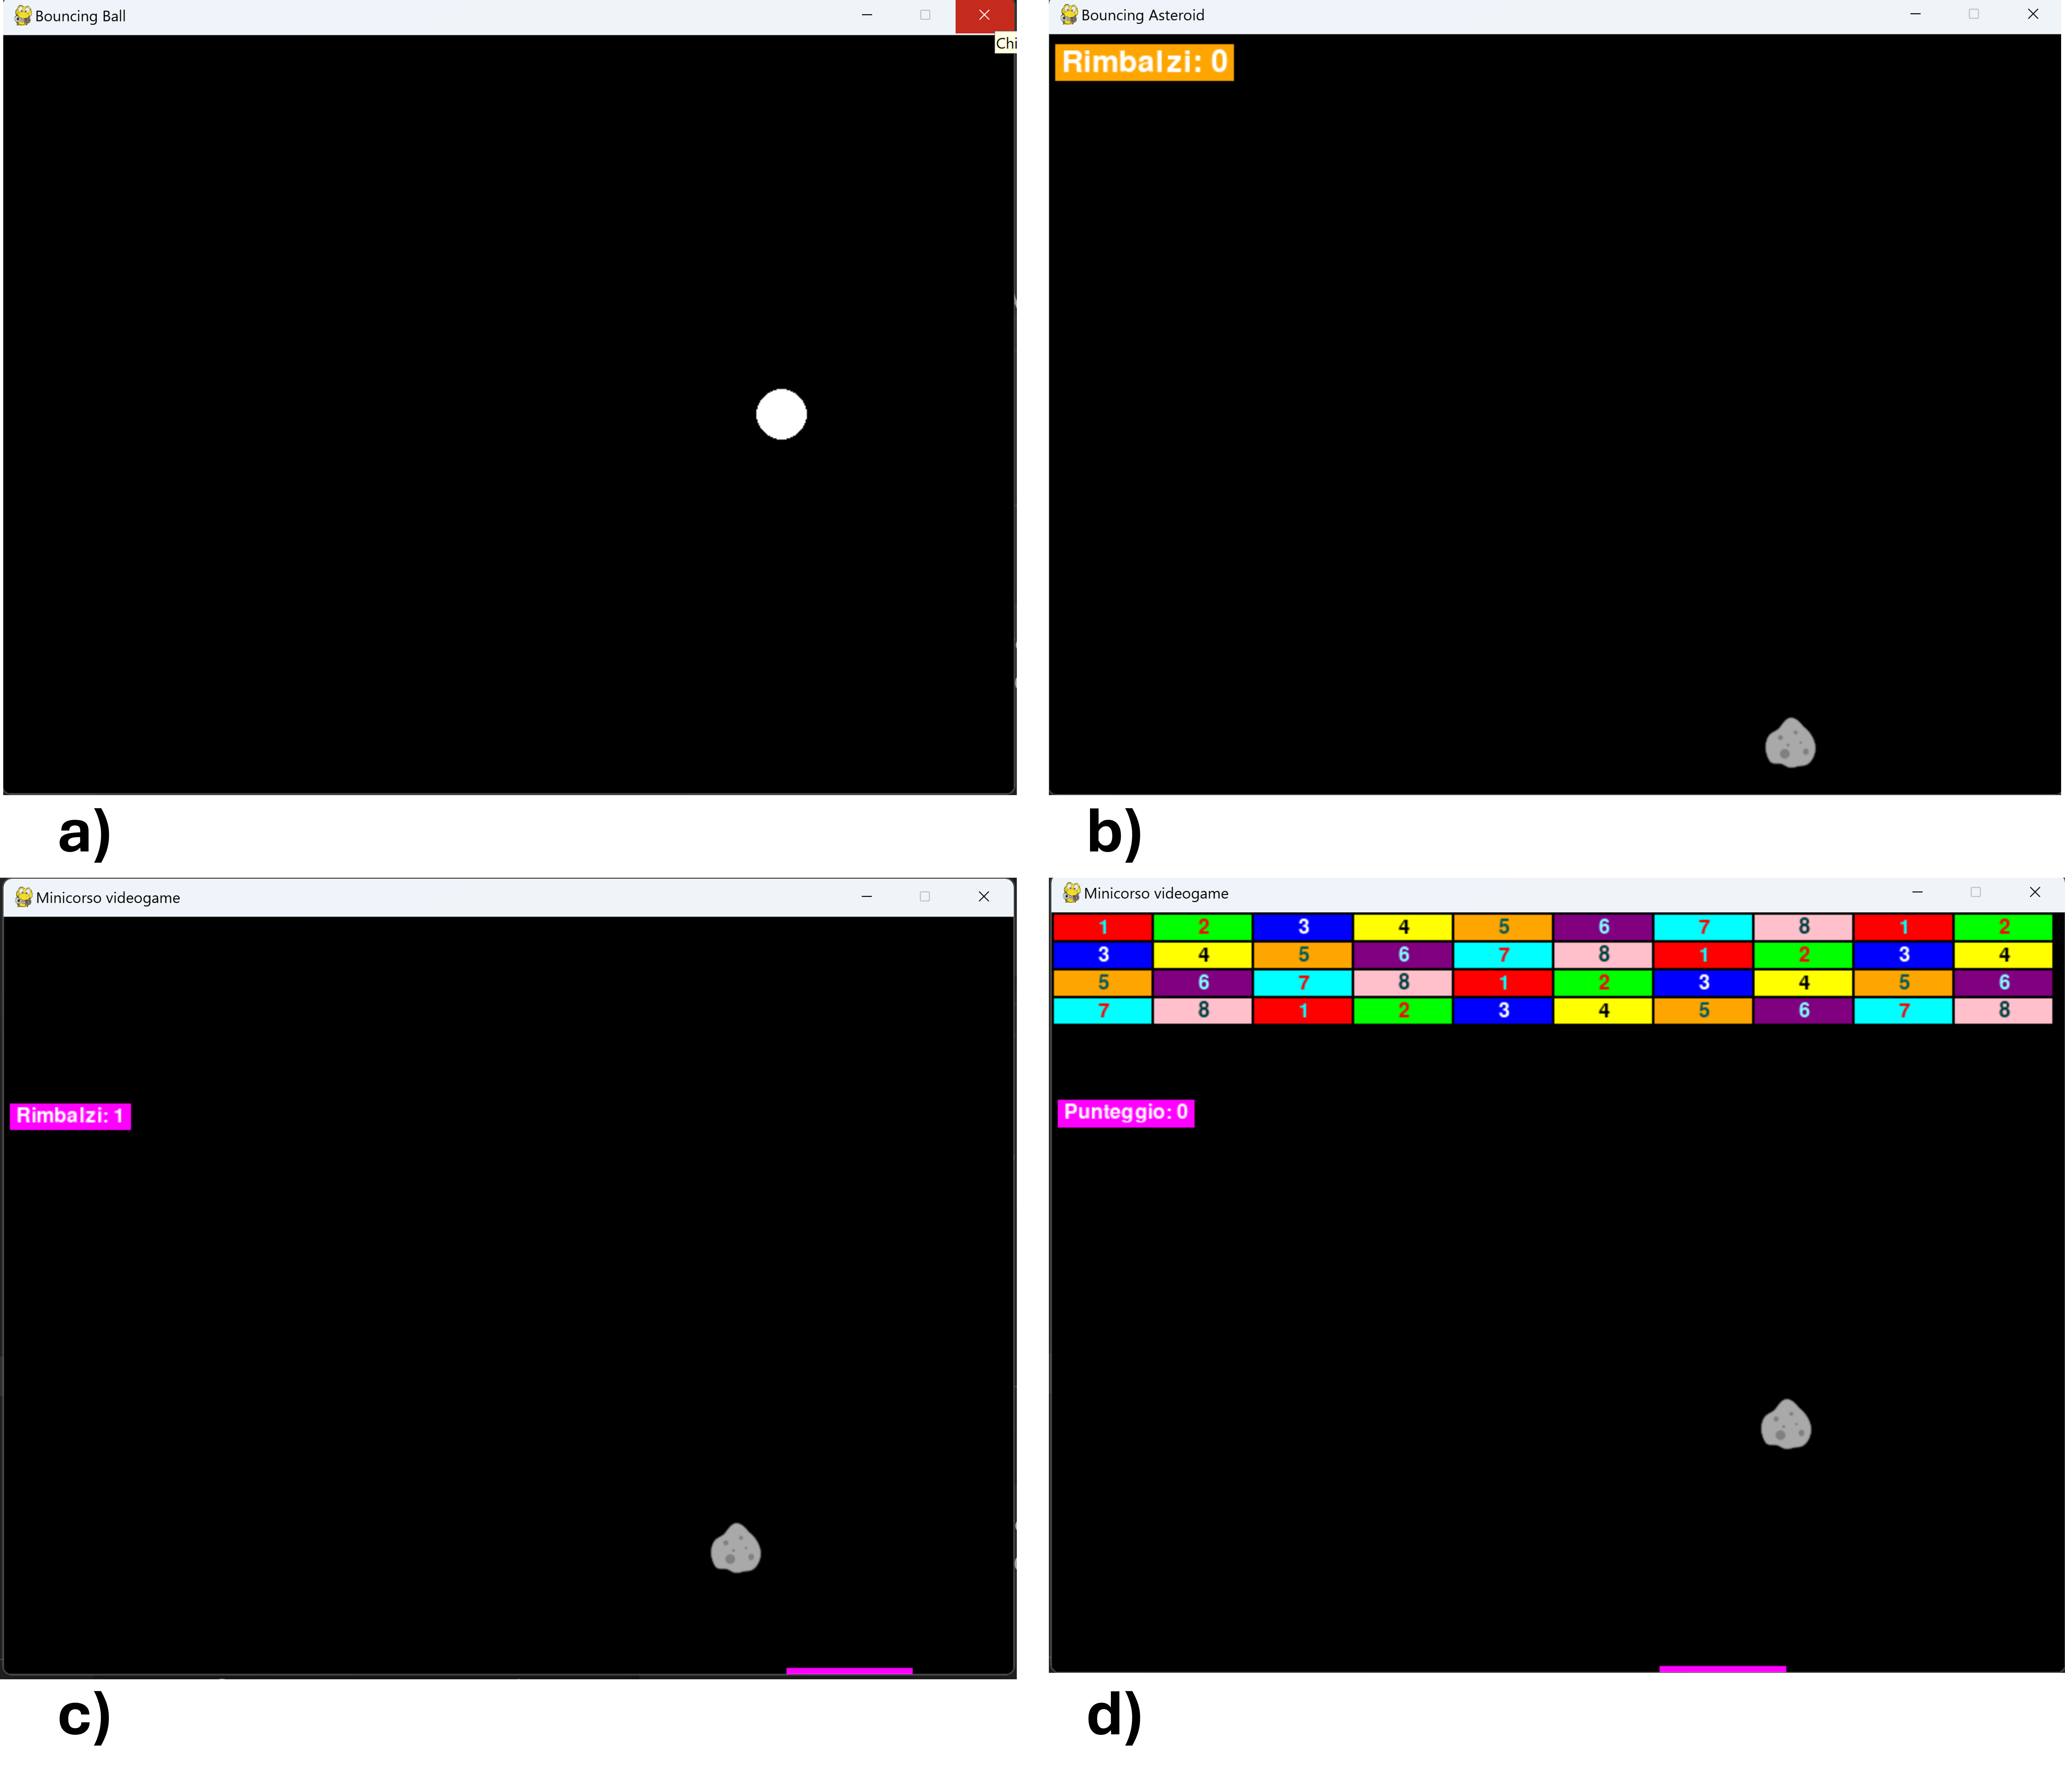
\includegraphics[width=1.0\textwidth]{game.png}
    \caption{a) animazione di un elemento all'interno della scena. b) rimbalzo di un elemento grafico complesso all'interno di una scena con audio contestuale. c) gestione del rimbalzo su una piattaforma mobile mediante \textit{arrow key}. d) logica completa di gioco con randomizzazione degli elementi (colore e punteggio).}
    \label{fig:game}
\end{figure}
Le realizzazione del gioco ha visto quattro momenti base. Il primo obiettivo è stato di realizzare una semplice scena introducendo un elemento grafico (cerchio) da muovere con una velocità costante; è stato fatto variare anche il valore di \textit{frame per second} per comprendere l'importanza di tale aspetto. Successivamente è stato introdotto un elemento grafico più complesso (immagine raster con sfondo trasparente) chiedendo di implementare logiche di rimbalzo con l'attivazione dell'audio contestualmente allo stesso. Successivamente si è posto l'accento sull'interazione dell'utente attraverso \textit{arrow keys} spostando una piattaforma nella parte inferiore del gioco, iniziando così ad implementare la parte centrale del gioco. Come ultimo sviluppo è stato chiesto di inserire degli elementi rettangolari a griglia con colori e valori \textit{random}; questa parte è sicuramente quella più complessa ed è stata completata in generale solo da un sotto-insieme di studenti e studentesse con una solida conoscenza di un linguaggio di programmazione.

\subsection{Competenze, Abilità e Conoscenze}
Il mini-corso è stato progettato nell'ottica di promuovere il potenziamento di competenze tecniche, trasversali e teoriche nell'ambito del mondo dei videogame. Al termine del corso, gli studenti hanno acquisito una panoramica sulle competenze preziose e trasversali, applicabili non solo nella progettazione di videogiochi ma anche in altre aree della tecnologia e del design.

\subsubsection{Competenze tecniche}
\begin{itemize}
    \item \textbf{Design grafico}: utilizzo di \texttt{Inkscape} per creare grafica vettoriale, progettazione di interfacce utente intuitive e visivamente accattivanti.
    \item \textbf{Acquisizione ed elaborazione numerica del suono}: tecniche di registrazione audio e possibilità creative fornite dai software utilizzati nel settore.
    \item \textbf{Programmazione}: conoscenze di base della programmazione in Python, utilizzo del framework \texttt{Pygame} per lo sviluppo di giochi, gestione delle collisioni e implementazione della fisica di base nel gioco.
\end{itemize}
\subsubsection{Competenze trasversali}
\begin{itemize}
    \item \textbf{Problem-solving}: abilità nel risolvere problemi complessi durante lo sviluppo del gioco, applicazione del pensiero logico e critico.
    \item \textbf{Collaborazione}: capacità di lavorare in gruppo, comunicare efficacemente con i compagni di squadra e condividere idee e soluzioni.
    \item \textbf{Creatività}: sviluppo della creatività attraverso la progettazione di interfacce, la creazione di grafica e la realizzazione di effetti sonori a partire dall'uso del corpo e da oggetti quotidiani.
\end{itemize}
\subsubsection{Conoscenze teoriche}
\begin{itemize}
    \item \textbf{Principi di game design}: comprensione delle basi del design di videogiochi e dell'importanza della UI e UX.
    \item \textbf{Fondamenti di audio per videogiochi}: conoscenza degli aspetti chiave dell'audio nel game design e orientamento rispetto alle esistenti tecniche di acquisizione e \textit{post-processing}.
    \item \textbf{Fondamenti di programmazione di videogiochi}: conoscenza di concetti base come rendering ed animazione di una scena, \textit{frame buffer} e \textit{frame per second} anche in ambiente Linux.
\end{itemize}
\section{Conclusioni}
\label{sec:conclusioni}

In conclusione, il corso "Come nasce un videogioco: aspetti di progettazione multimediale audio-video ed interfacce" ha offerto agli studenti e studentesse un'esperienza formativa che riteniamo essere stata completa e coinvolgente. Attraverso un approccio laboratoriale e interattivo, gli studenti e le studentesse hanno imparato a riconoscere quali sono le competenze tecniche necessarie per affrontare il mondo dei videogame dove più che mai è necessario confrontarsi con sfide multidisciplinari. Sicuramente i tempi previsti, ovvero 15h, si sono rivelati ridotti rispetto alle necessità di uno sviluppo completo ed in autonomia. Il corso è stato erogato a studenti e studentesse che spaziano dal primo al quinto anno; la conoscenza pregressa di un linguaggio di programmazione si è dimostrata di notevole utilità aumentando il grado di raggiungimento degli obiettivi iniziali; vale la pena rimarcare comunque che l'utilizzo di un linguaggio come Python abbia semplificato il processo di scrittura del codice.

\section*{Acknowledgements}
Gli autori desiderano ringraziare anche la Prof.ssa Patrizia Melli (Istituto di Istruzione Superiore Cambi Serrani) e la Prof.ssa Federica Minni (Istituto Istruzione Superiore Savoia Benincasa) per il loro supporto nell'organizzare le attività di orientamento presso i rispettivi istituti. Si ringrazia inoltre il Prof. Domenico Ursino dell'Università Politecnica delle Marche per aver contribuito all'istituzione del corso di laurea triennale in Ingegneria dell'Informazione per Videogame e Realtà Virtuale.

\label{sect:bib}
\bibliographystyle{plain}
%\bibliographystyle{alpha}
%\bibliographystyle{unsrt}
%\bibliographystyle{abbrv}
\bibliography{game}
\end{document}